\question[10] A partir de los datos de en cada figura, encuentra la medida del \'angulo $x$ para cada uno de los siguientes incisos.
%\begin{multicols}{2}
   
    \begin{minipage}[b]{0.43\textwidth}
        \begin{figure}[H]
            \caption{Diagrama geométrico donde se encuentra la inc\'ognita $x$.}
            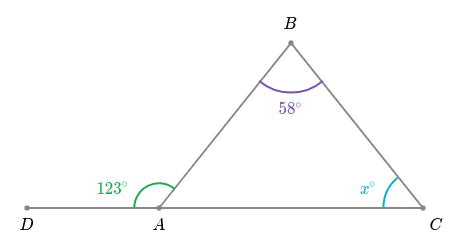
\includegraphics[width=\linewidth]{Images/triangle_angle_01}
            \label{fig:triangle_angle_01}
        \end{figure}
        {
        \color{cielo}\textbf{$\angle x^\circ =$}} \fbox{
        \begin{minipage}{2cm}
            \hfill\vspace{0.5cm}
        \end{minipage}
    }
    \end{minipage}
    \hspace{2cm}
    \begin{minipage}[b]{0.43\textwidth}
        \begin{figure}[H]
            \caption{Diagrama geométrico donde se encuentra la inc\'ognita $x$.}
            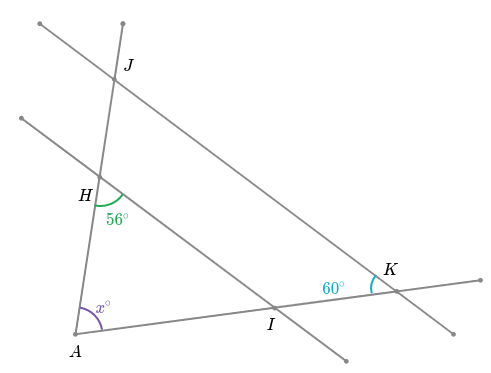
\includegraphics[width=\linewidth]{Images/triangle_angle_04}
            \label{fig:triangle_angle_04}
        \end{figure}
        {
            \color{purplePoint}\textbf{$\angle x^\circ =$}} \fbox{
            \begin{minipage}{2cm}
                \hfill\vspace{0.5cm}
            \end{minipage}
        }
    \end{minipage}
%\end{multicols}